\documentclass[12pt]{article}
\usepackage{times}
\usepackage{plext}
\usepackage{cite}
\usepackage{setspace}
\usepackage{float}
\usepackage{lineno}
\usepackage{color}
\usepackage[dvipdfmx]{graphicx}
\usepackage{array, booktabs}
\usepackage[top=25truemm,bottom=25truemm,left=30truemm,right=30truemm]{geometry}
\usepackage{threeparttable}
\usepackage{ulem}
%\usepackage{amsmath}
\renewcommand{\figurename}{Fig.}
\renewcommand{\tablename}{Table}
\begin{document}\setcounter{page}{1}
\renewcommand\citeleft{(} 
\renewcommand\citeright{)}

\flushleft{\textbf{Title: Inetgrated spatial model estimates the fish distribution using environmental DNA and catch data}}\\
%\flushleft{\textbf{Running title: }}\\
\flushleft{Yuki Kanamori$^{1\ast}$, Hiroshi Okamura$^{2}$, Shota Nishijima$^{2}$, Yuki Hongo$^{2}$, Yasuyuki Uto$^{3}$, Hisatoku Mita$^{4}$, Mitsuhiyo Ishii$^{4}$, Kiyoharu Akimoto$^{5}$, and Akane Kusano$^{6}$}\\
\ \\
$^{1}$ Fisheries Resources Institute, Japan Fisheries Research and Education Agency, 25-259 Shimomekurakubo, Samemachi, Hachinohe, Aomori 031-0841, Japan\\
$^{2}$ Fisheries Resources Institute, Japan Fisheries Research and Education Agency, 2-12-4 Fukuura, Kanazawa, Yokohama, Kanagawa 236-8648, Japan\\
$^{3}$ \\
$^{4}$ \\
$^{5}$ \\
$^{6}$ \\
\ \\

$^{\ast}$ Corresponding author\\
Email: kana.yuki@fra.affrc.go.jp

\newpage
\flushleft{\textbf{Abstract}\\}

\flushleft{\textbf{Keywords}}\\

\newpage
\begin{linenumbers}
\setstretch{2}
\section{Introduction}
Understanding of spatial distribution of species and underling its mechanism is a essential issue in ecology.
Field surveys using environmental DNA (eDNA) are widely used for detecting invasive or rare species and hotspot of biodiversity (面倒なのでレビュー論文を引用) because the surveys of eDNA are easy to detect presence/absence of target species, non-invasiveness, and high cost effectiveness rather than previous direct sampling method (Rees et al. 2014; Thomsen \& Willerslev 2015 %Dorazioに引用されていたやつ.あとで再確認).
%Field survey using eDNA is easy to detect presence/absence of target species, non-invesiveness, and high cost effectiveness rather than previous direct sampling methods such as visual or aural, so that eDNA is widely used to detect invesive species, rare species, and hot spot of biodiversity.
However, the presence/absence of eDNA includes many types of uncertainties due to relating to environmental factors such as temperature and advection ().
For example, in aquatic habitats, it is not sure whether target species are in a location or not when eDNA of target species is detected because eDNA are transported passively.
Therefore, the consideration to the influence of environmental factors on eDNA is necessary for estimation of species distribution when we use eDNA methods.

\ \ \ \ \ \ \ \ \ \ 
One step towards overcoming these uncertainties is a understanding of the "ecology of eDNA":  (Barnes \& Turner 2016). Previous studies

\ \ \ \ \ \ \ \ \ \ 
Integrated species distribution models (IDMs) are now common spatial model to predict spatial pattern of species (Issac et al. 2020).
The model use the different type of data with strengths and weaknesses, such as scientific survey data which is restricted spatially and quantitatively and opportunistic citizen data which is widely collected and abundant, and combine in a single model (Isaac et al. 2020; Miller et al. 2019).

The models combine the different type of data with strengths and weaknesses in a single model ().
For example, scientific survey data are high quality but less abundant due to restriction of spatially costly while opportunistic data such as citizen data are widely collected and abundant but may be low quality due to not using consistent field methods.
Combining both types of data can capitalize on the strengths of each data and perform better prediction than models when we use single data (Pacifici et al. 2017; Miller et al. 2019).



\ \ \ \ \ \ \ \ \ \ 
Tokyo Bay is a large enclosed coastal sea in Japan. In Tokyo Bay, there are many commercially important species for fisheries that are called "Edomae" because these species have been used for Sushi since Edo Era (about 400 years ago). Catch of some Edomae have been decreased because of habitat modification due to urbanization (e.g., landfill of tidal flats and water pollution). Catch statistics (total catch in each species, efforts, and geographic location of fishing) have been collected for stock assessment since 1990 by prefectures around Tokyo Bay. The strengths of this data are the direct evidence that a focal species occupies a location of fishing and abundant because of widely collected in Tokyo Bay.  On the other hand, weakness of this data is like a opportunistic data because the data is likely to be biased towards areas to high density of focal species due to commercially fishes, consequently less zero data. In addition to this catch statistics, scientific survey of eDNA has been conducted monthly since 2018 for biodiversity monitoring because biodiversity also may decreased due to human-induced environmental changes in Tokyo Bay (Hongo et al., submitted). The strengths are that the data is systematically collected by scientific survey data and includes zero data, while the weaknesses are that the data is less abundant due to spatial restriction of the survey and includes uncertainties in presence/absence as description in above.


\ \ \ \ \ \ \ \ \ \ 
In this paper, to predict spatial distribution of species from eDNA, we first make a model which considers uncertainties of eDNA caused by environmental factors without additional laboratory experiments and numerical hydrodynamic models, by using an integrated spatial distribution model (eDNA-IDM). We then apply the model to both eDNA data and catch statistics for four Edomae fish in Tokyo Bay, Japan. 
The predicted spatial distribution of four fish form our model reduced 

%In this paper, we make an integrated spatial distribution model by combining both catch statistics, which is opportunistic data but abundant and represents the direct evidence where fish was, and eDNA data, which is the monitoring data in the same points but not abundant and includes uncertinties due to environmental factors.

%In this paper, we make the model considering with uncertinties caused by environmental factors, such as temperature and advection, to predict spatial distribution of species using an integrated spatial distribution model. 

\ \\

\section{Materials and Methods}
%2.1: a general model to estimate species distribution from eDNA
%2.2: an application to a eDNA and catch data in Tokyo Bay
%2.2.1: 野外調査
%2.2.2: 漁獲量データ
%2.2.3: model in Tokyo Bay


\subsection{A general model to estimate species distribution from eDNA}
Integrated spatial distribution model that account for explicitly spatial autocorrelation in occurrence were built by Pacifici et al. (2017), which shows three approaches to predict the spatial distribution of species: the joint likelihood (shared), correlation, and covariate methods. The joint likelihood method uses multiple data types to simultaneously estimate a shared set of parameters with constraining that the likelihoods of shared set of parameters to be equal across. The correlation method connects multiple data types indirectly through a shared covariance matrix that captures similar patterns present in each data sources. The covariate method incorporates information from a added dataset via a fixed effect. 

\ \ \ \ \ \ \ \ \ \ 
Although each methods estimate the spatial distribution of species using multiple data sets, we need to select method depending on the data features for analysis because there are strengths and weaknesses (Pacifici et al. 2017; Miller et al. 2018). The joint likelihood method may be problematic when the second data is of poorly quality compared to correlation and covariate methods because each data can directly inform the latent occurrence state (probabilities?) and the weight given to estimate the parameters is naturally determined by their relative size and quality. Thus, it is not the best method when our second data is low quality while it is the best method when our second data is high quality (vise versa). 
%The joint likelihood method simultaneously fits a likelihood to both data sources
%The joint likelihood approach uses multiple data types to simultaneously estimate a shared set of parameters.
%the shared set of parameters within each of the individual likelihoods is constrained to be equal across likelihoods.
The correlation method is added robustness to the joint likelihood because the second data indirectly inform the occurrence state. Thus, it is the best method when our second data is low quality while it is inferior to the joint likelihood method when both data are deemed reliable.
%The correlation method is added robustness to the joint likelihood for the influence of unreliable data because the second data indirectly inform the occurrence state.
% while this method is inferior to the joint likelihood when both data are deemed reliable.  


\ \ \ \ \ \ \ \ \ \ 
In this study, to estimate the spatial distribution of species from eDNA considering with spatial uncertainties, we make a integrated species distribution model using correlation method.

\[
\mathrm{logit}(p_{1}(s_{i})) = \alpha_{1} + \beta(s_{i}) + \theta(s_{i}) + u_{1}(s_{i})
\]
\[
\mathrm{logit}(p_{2}(s_{i})) = \alpha_{2} + \sum_{k}f_{k}(x_{k}(s_{i})) + w \theta(s_{i}) + u_{2}(s_{i})
\]
%\flushleft{\textbf{2.1.1 Survey and data}}\\
%The egg density data with $\textrm{30}^\prime$ latitude $\times$ $\textrm{30}^\prime$ longitude horizontal square resolution in the areas from $\textrm{122}^\circ$E to $\textrm{150}^\circ$E and $\textrm{24}^\circ$N to $\textrm{43}^\circ$N was used. The egg density data set was derived from monthly egg surveys off the Pacific coast of Japan from January to June, 2005--2019 (Takasuka et al., 2008a, 2019). The aim of the surveys was to monitor the egg abundance of major small pelagic fish species, including chub mackerel and spotted mackerel, so that the spatial area and survey month of the data largely covered the major spawning grounds and spawning season. While some sampling locations were fixed, others varied for various reasons (e.g., environmental conditions). Accordingly, the survey design changed slightly each year (Kanamori et al., 2019). Although the sampling efforts were approximately consistent year-round, the efforts tended to be more intensive during early spring; effort was highest in February and decreased gradually thereafter (Takasuka et al., 2008b). 

%\ \ \ \ \ \ \ \ \ \ 
%The egg surveys were conducted by 18 prefectural experimental stations or fisheries research institutes and two national research institutes of the Japan Fisheries Research and Education Agency, following the consistent sampling designs, as a part of the stock assessment project. In the surveys, plankton nets were towed vertically from a depth of ~150 m to the surface (if the depth was <150 m, nets were lowered to just above the bottom). This range of depths covers the vertical distributions of eggs of small pelagic fish. During the period from 2005 to 2019, the surveys used a plankton net with a mouth ring diameter of 0.45 m and a mesh size of 0.335 (partially 0.330 mm in 2015) (Takasuka et al., 2017). The samples were fixed with 5\% formalin immediately after collection. In the laboratory, the samples were identified and sorted into eggs and larvae of different small pelagic species, based on the morphological characteristics (e.g., egg shape and size, number of oil globules, segmented yolk, perivitelline space ranging, yolk diameter, oil globule diameter). For the mackerel eggs, the egg diameters were measured to the nearest 0.025 mm by a micrometer for a maximum number of 100 individuals per sample (station or tow). Eggs with diameters $>$1.1 mm were identified as spotted mackerel, whereas those with diameters $leq$1.0 mm were identified as chub mackerel, according to Nishida et al. (2001). For any sample of $>$100 individuals, the proportion of the two species among 100 randomly selected individuals was assumed to be the same for the whole sample. Additionally, the number of eggs per unit area in the water column (number $\mathrm{m^{-2}}$) for each sampling tow was calculated by flow-meter revolutions, flow-meter revolutions per meter tow in the calibration, wire length (m), opening mouth area of the net  ($\mathrm{m^{-2}}$), and wire angle. Then, the arithmetic average of the number of eggs was obtained with $\textrm{30}^\prime$ latitude $\times$ $\textrm{30}^\prime$ longitude horizontal square resolution. 
%\textcolor{red}{The mean proportion of the total number of eggs of spotted mackerel against the total number of eggs of \textit{Scomber} was less than 20 \% from 2005 to 2019. Therefore, the effect of the misidentification error that we considered was from chub mackerel on spotted mackerel (i.e., we assumed that the effect of the misidentification error from spotted  mackerel on chub mackerel was small.)} More detailed descriptions of the surveys and data set are provided in previous studies of the reproductive biology of small pelagic fish species (e.g., Takasuka et al. 2008a,b, 2017, 2019).


\subsection{An application to a eDNA and catch data in Tokyo Bay}
\flushleft{\textbf{2.2.1 eDNA data}}\\
\flushleft{\textbf{Field surveys}}\\
Field surveys were conducted by prefectural experimental station in Chiba, following the consistent sampling design at 14 sites in Tokyo Bay from April to December in 2018 (Fig. 1). 
%Field surveys were conducted at 14 sites in Tokyo Bay from April to December in 2018 using R/V Fusanami or R/V Fusami-maru of Chiba Prefecture and R/V Enoshima-maru of Kanagawa Prefecture (Fig. 1). 
In each sites, seawater and environmental data were simultaneously collected. For eDNA analysis, two litter of bottom seawater was collected using a Niskin water sampler, and then it was separated for two 1L samples for replicate. Each samples filtered glass fiber membrane GF/F (0.7 $\mu m$ pore size; Cytiva, Sheffield, UK) onboard and then the filters were frozen on a block of dry ice. These frozen filters were stored at $-30^\circ$ in the laboratory until eDNA extraction. To lower the levels of cross-contamination, equipments for eDNA sampling were changed new one or washed in each sites. During sampling the bottom seawater, seawater temperature, salinity, pH, and dissolved oxygen (DO) at the same depth of seawater sampling for eDNA were measured by CTD (メーカー).
%The egg surveys were conducted by 18 prefectural experimental stations or fisheries research institutes and two national research institutes of the Japan Fisheries Research and Education Agency, following the consistent sampling designs, as a part of the stock assessment project.

\flushleft{\textbf{Laboratory experiments}}\\
In laboratory, eDNA extraction, eDNA amplification, and eDNA sequence were conducted. Total eDNA was extracted from the frozen filters using a DNeasy Blood and Tissue Kit (Qiagen, Hilden, Germany) following Yamamoto et al. 2019. Mitochondorial 12S rRNA gene was amplified using MiFish universal primers referring to Miya et al. 2015 with slight modification. The details was shown in Hongo et al. (受理されてないようだったら書くしかない).  eDNA sequence were ....


\flushleft{\textbf{2.2.2 Catch statistics}}\\
A part of catch statistics of small-scale bottom trawl fisheries recorded by several representative boats of Chiba Prefecture were provided by Chiba Prefecture. This data included date, geographic location, efforts (number of tows), gear, and catch weight (kg) in each fish. Almost of all gear was beam trawl although dredge net also used. The species which also detected by eDNA was \textit{Conger myriaster} (マアナゴ), \textit{Kareius bicoloratus} (イシガレイ), \textit{Lateolabrax japonicus} (スズキ), and \textit{Konosirus punctatus} (コノシロ). Thus, we estimated the spatial distribution of these four species using the eDNA-IDM. \textcolor{red}{マコガレイ,カマス類,クロダイ,イシモチ類も解析できる??}

\flushleft{\textbf{2.2.3 Estimation of spatial distribution}}\\
To estimate the spatial distribution of four focal species from eDNA and catch data by considering uncertainties caused by environmental factors, we fitted the model (equation 1) to the presence/absence data of eDNA and of catch data collected in Tokyo Bay as follows:



\flushleft{\textbf{equation examples}}\\
%\[
\begin{equation}
\begin{array}{ll}
\mathrm{logit}\ p_{i} = \beta_{p}(t_{i}) + \omega_{p}(s_{i}) + \varepsilon_{p}(s_{i}, t_{i}) + \eta_{p}(v_{i}) + \lambda_{p}Q(i)\\
%\]
%\[
\log d_{i} = \beta_{d}(t_{i}) + \omega_{d}(s_{i}) + \varepsilon_{d}(s_{i}, t_{i}) + \eta_{d}(v_{i}) + \lambda_{d}Q(i)
%\]
\end{array}
\end{equation}
where $\beta(t_{i})$ is the intercept for year $t$, and $\omega(s_{i})$ and $\varepsilon(s_{i}, t_{i})$ are the spatial and spatio--temporal random effects for year $t$ and location $s$, respectively. $\eta(v_{i})$ is the overdispersion random effect of factor $v_{i}$, which is the interaction of year and month. 
$\lambda$ is the effect of the chatchability covariate $Q(i)$: 
\[
%Q(i) = \mathrm{log} (\mathrm{chub\,mackerel\,egg\,density}(s_{i})+0.1). 
Q(i) = \mathrm{log} (d_{chub}(s_{i})+0.1). 
\]
That is, this term considers the effect of species misidentification between chub mackerel and spotted mackerel; as mentioned earlier, we suspected overestimation of egg density of spotted mackerel because the difference in egg diameter has become ambiguous according to increase in egg density of chub mackerel and the distributions of egg diameters between species have overlapped (Yukami et al., 2019). The constant 0.1 was added because $\mathrm{log} 0$ (i.e., no chub mackerel eggs) is undefined, and the same result was obtained when using $1$ in place of $0.1$.



\ \\
%\setstretch{1}
\flushleft{\textbf{\Large{Acknowledgments}}}\\
This research was financially supported by Grant-in-Aid for Fisheries Agency of Japan.
%This research was financially supported by the grants from the Japan Society for the Promotion of Science (JSPS) (19K15905, 20392904).
\ \\

\flushleft{\textbf{\Large{Authorship}}}\\
YK conceived of the research idea. YH, YU, HM, MI, KA, and AK conducted field sampling. YH performed the laboratory experiments. YK, HO, and SN designed statistical analyses. YK wrote programs and performed the analyses. YK wrote the manuscript with input from all co-authors' comments.
\ \\

\newpage
\begin{figure}[h]
  \centering
  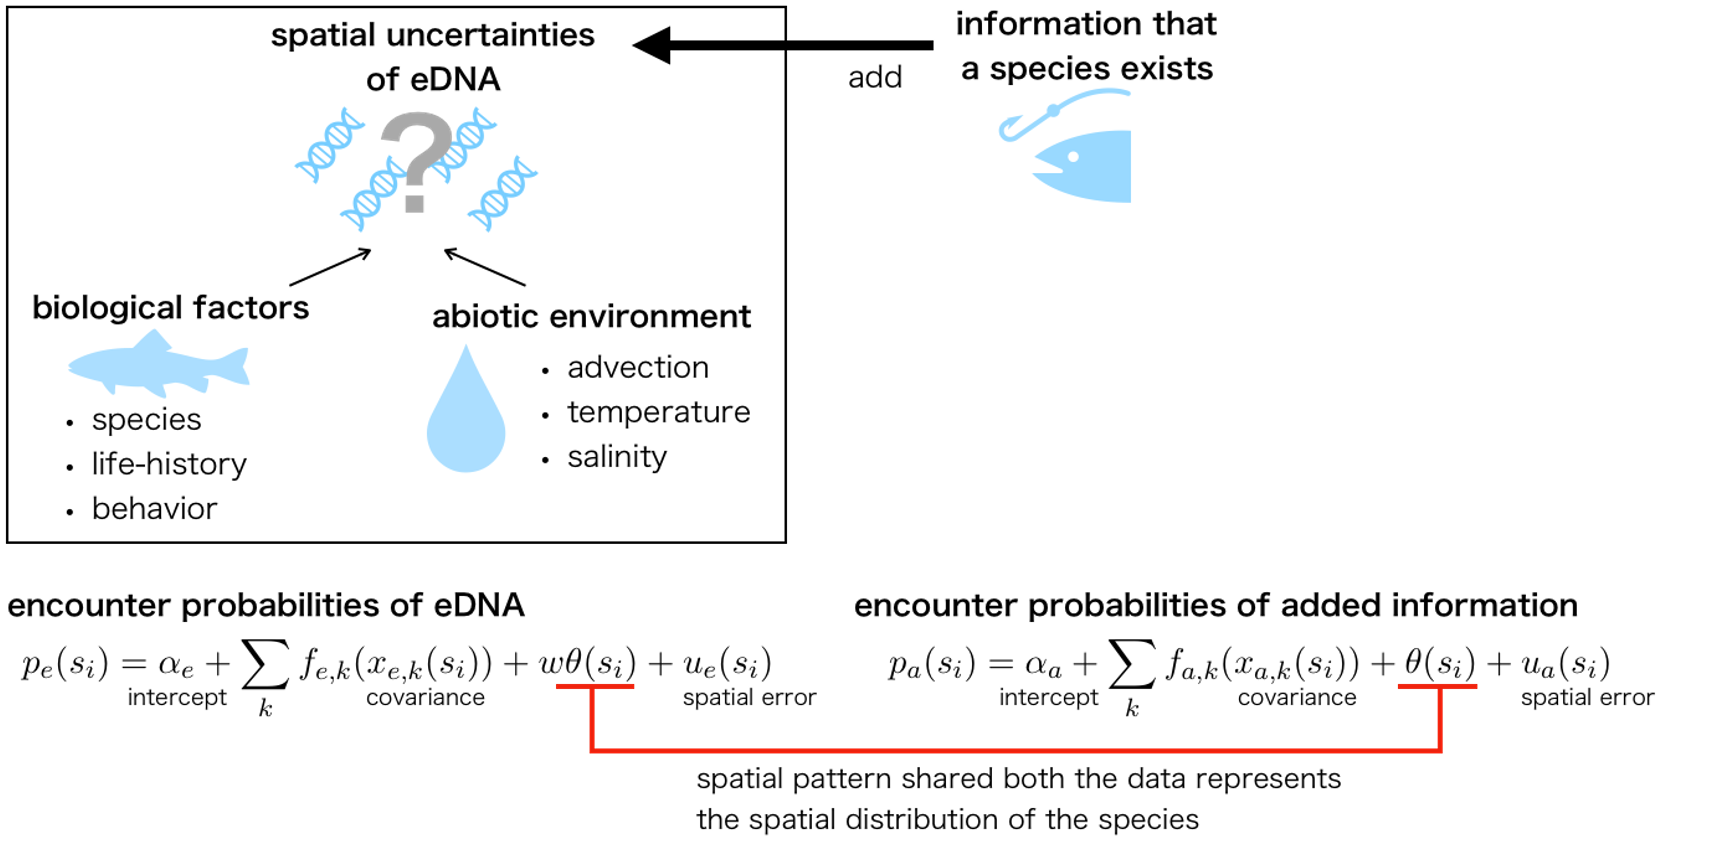
\includegraphics[width = 18cm]{idea.png}
  \caption{Conceptual diagram of this study.}
\end{figure}



\end{linenumbers}
\end{document}
